\documentclass[titlepage, a4paper, 12pt, reqno, openany]{report}
%\documentclass[12pt]{report}
%\documentclass[titlepage, a4paper, 12pt, reqno, openany]{article}
%\documentclass[12pt]{article}
%%%%%%%%%%%%%%%%%%%%%%%%%%%%%%%%%%%%%%%%%%%%%%%%%%%%%%%%%%%%%%%%%%%%%%%%%%%%%
\usepackage{titlepic}
%%%%%%encoding%%%%%%
\usepackage[T1]{fontenc}
\usepackage[utf8]{inputenc}
\usepackage[portuguese]{babel}
\usepackage{hyphenat}
%\usepackage{hyphsubst}
%%%%%%Hyphenation rules%%%%%%
\usepackage{graphicx} %permite inserir figuras
\usepackage{caption} %titulo graphicos
\usepackage[font=small,labelfont=bf]{caption} %reference figures
%\usepackage{subcaption}
\usepackage{color,colortbl}
\usepackage[usenames,dvipsnames,svgnames,table]{xcolor} %permite letras coloridas
\usepackage[top=2cm,left=1.5cm,right=1.2cm,bottom=2cm]{geometry}
%\usepackage[margin=2cm]{geometry} %margens
%\usepackage[left=2cm,top=1cm,bottom=2cm,right=3cm,nohead,nofoot]{geometry}
\usepackage{paralist}
\usepackage{float}
\usepackage{verbatim}
\usepackage{lipsum}
\usepackage{multicol}
\usepackage{multirow}
\usepackage{makecell}
\usepackage{babelbib}
%\usepackage{biblatex}
\usepackage{amsfonts}
\usepackage{amsmath}
\usepackage{amssymb}
%%%%%%%%%%%%%%%%%%%%%%%%%%%%%%%%%%%%%%%%%%%%%%%%%%%%%%%%%%%%%%%%%%%%%%%%%%%%%%%
\usepackage[export]{adjustbox}
\usepackage{lipsum}
%\usepackage{adjustbox}
\usepackage{setspace} %distancia entree linhas
\usepackage{eurosym}
%\usepackage[table,xcdraw]{xcolor}
%\usepackage{times}
%\usepackage{makeidx} %para criar índice remissivo
%\usepackage{array}
%\usepackage{supertabular}
%\usepackage{bm}
%\usepackage{booktabs}
%\usepackage{boxedminipage}
%\usepackage{caption}
%\usepackage{changepage}
%\usepackage{cite}
%\usepackage{easylist}
%\usepackage{esint}
%\usepackage{eucal}
%\usepackage{fancyhdr}
%\usepackage{hyperref} %index dentro de red boxes
%\usepackage{indentfirst}
%\usepackage{latexsym}
%\usepackage{listings}
%\usepackage{mathptmx}
%\usepackage{mathrsfs} %permite o uso de letras trabalhadas
%\usepackage{microtype}
%\usepackage[normalem]{ulem} %permite sublinhar palavras
%\usepackage{pifont}
%\usepackage{rotating}
%\usepackage{setspace}
%\usepackage{syntonly} %speedup work desabling pdf converse \syntaxonly
%\usepackage{subfiles}
%\usepackage{textcomp}
%\usepackage{theorem}
%\usepackage{ulem}
%\usepackage{url}
%\usepackage{wrapfig}
%%%%%recent%%%%%
%\usepackage{cancel}
%\usepackage[fleqn]{mathtools}
%\usepackage{pdfpages}
%\usepackage{pdflscape}
%\usepackage{todonotes}
%\usepackage{siunitx}
%%%%%%%%%%%%%%%%%%%%%%%%%%%%%%%%%%%%%%%%%%%%%%%%%%%%%%%%%%%%%%%%%%%%%%%%%%%%%%%%%%%
%\renewcommand\thesection{\arabic{section}}
%\renewcommand\thesubsection{\thesection.\arabic{subsection}}
%%%%%%%%%%%%%%%%%%%%%%%%%%%%%%%%%%%%%%%%%%%%%%%%%%%%%%%%%%%%%%%%%%%%%%%%%%%%%%%%%%%%
\usepackage{enumitem}
\begin{comment}
\setlistdepth{12}
\newlist{enumitem}{enumerate}{12}
\setlist[enumitem,1]{label=\roman*)}
\setlist[enumitem,2]{label=\alph*)}
\setlist[enumitem,3]{label=\arabic*)}
\setlist[enumitem,4]{label=(\roman*)}
\setlist[enumitem,5]{label=(\alph*)}
\setlist[enumitem,6]{label=(\arabic*)}
\setlist[enumitem,7]{label=\roman*)}
\setlist[enumitem,8]{label=\alph*)}
\setlist[enumitem,9]{label=\arabic*)}
\setlist[enumitem,10]{label=(\roman*)}
\setlist[enumitem,11]{label=(\alph*)}
\setlist[enumitem,12]{label=(\arabic*)}
\end{comment}

%%%%%%%%%%%%%%%%%%%%%%%%%%%%%%%%%%%%%%%%%%%%%%%%%%%%%%%%%%%%%%%%%%%%%%%%%%%%%%%%%%%%
\begin{comment}
\usepackage{enumerate}
\renewcommand{\labelitemi}{$\bullet$}
\renewcommand{\labelitemii}{$\cdot$}
\renewcommand{\labelitemiii}{$\diamond$}
\renewcommand{\labelitemiv}{$\ast$}
\end{comment}

%%%%%%%%%%%%%%%%%%%%%%%%%%%%%%%%%%%%%%%%%%%%%%%%%%%%%%%%%%%%%%%%%%%%%%%%%%%%%%%%%%%%
\begin{comment}
\usepackage{tikz}
\usepackage{circuitikz}
\usetikzlibrary{matrix,shapes.geometric,arrows,trees,positioning,calc}
%%%%%%%%%%%%%%%%%%%%%%%pre defined figures%%%%%%%%%%%%%%%%%%%%%
\tikzstyle{RECTANGLE_2} = [rectangle, draw, text width=5em, text centered, rounded corners, minimum height=4em]
\tikzstyle{RECTANGLE_3} = [rectangle, rounded corners, minimum width=3cm, minimum height=1cm,text centered, draw=black, fill=red!80]
\tikzstyle{RECTANGLE_4} = [rectangle, draw, fill=blue!20, text width=3cm, text centered, minimum height=4em]
\tikzstyle{RECTANGLE_5} = [rectangle, minimum width=3cm, minimum height=1cm, text centered, text width=3cm]
\tikzstyle{RECTANGLE_6} = [rectangle, draw, fill=blue!20, text width=5em, text centered, rounded corners, minimum height=4em]
\tikzstyle{RECTANGLE_7} = [rectangle, draw, fill=blue!20, text width=5em, text centered, rounded corners, minimum height=4em]
\tikzstyle{RECTANGLE_8} = [rectangle, draw, align=left, fill=blue!20]
\tikzstyle{RECTANGLE_1} = [rectangle, rounded corners, minimum width=1cm, minimum height=1cm,text centered, draw=black, fill=green!%30]
\tikzstyle{DIAMOND_1} = [diamond, draw, fill=blue!20, text width=4.5em, text badly centered, node distance=4cm, inner sep=0pt]
\tikzstyle{DIAMOND_2} = [diamond, minimum width=3cm, minimum height=1cm, text centered, draw=black, fill=green!30]
\tikzstyle{DIAMOND_3} = [diamond, draw, text width=4.5em, text badly centered, node distance=3cm, inner sep=0pt]
\tikzstyle{DIAMOND_4} = [diamond, draw, fill=blue!20, text width=4.5em, text badly centered, node distance=3cm, inner sep=0pt]
\tikzstyle{DIAMOND_5} = [diamond, draw, fill=blue!20, text width=4.5em, text badly centered, node distance=3cm, inner sep=0pt]
\tikzstyle{DIAMOND_6} = [diamond, draw, fill=blue!20, text width=4.5em, text badly centered, node distance=4cm, inner sep=0pt]
\tikzstyle{DIAMOND_7} = [diamond, draw, align=left, fill=blue!20]
\tikzstyle{ELLIPSE_1} = [draw, ellipse,fill=red!20, node distance=3cm, minimum height=2em]
\tikzstyle{ELLIPSE_2} = [draw, ellipse,fill=red!20, node distance=3cm, minimum height=2em]
\tikzstyle{ELLIPSE} = [draw, ellipse,fill=red!20, node distance=3cm, minimum height=2em]
\tikzstyle{TRAPEZIUM_1} = [trapezium,trapezium left angle=70,trapezium right angle=-70,minimum height=0.6cm, draw, fill=blue!20, text width=4.5em, text badly centered, node distance=3cm, inner sep=0pt]
\tikzstyle{TRAPEZIUM_2} = [trapezium, trapezium left angle=70, trapezium right angle=110, minimum width=3cm, minimum height=1cm, text centered, draw=black, fill=blue!30]
\tikzstyle{TRAPEZIUM_3} = [trapezium,trapezium left angle=70,trapezium right angle=-70,minimum height=0.6cm, draw, fill=blue!20, text width=4.5em, text badly centered, node distance=3cm, inner sep=0pt]
\tikzstyle{ARROW} = [thick,->,>=stealth]
\tikzstyle{LINE} = [draw, -latex']
\tikzstyle{MYLINE} = [draw, ->,  thick, shorten <=4pt, shorten >=4pt]
\tikzstyle{TEXT_1}=[draw,text centered,minimum size=6em,text width=5.25cm,text height=0.34cm]
\tikzstyle{TEXT_2}=[draw,text centered,minimum size=2em,text width=2.75cm,text height=0.34cm]
\tikzstyle{TEXT_3}=[draw,minimum size=2.5em,text centered,text width=3.5cm]
\tikzstyle{TEXT_4}=[draw,minimum size=3em,text centered,text width=6.cm]
\tikzstyle{CIRCLE_1}=[draw,shape=circle,inner sep=2pt,text centered, node distance=3.5cm]
\tikzstyle{CIRCLE_2}=[draw,shape=circle,inner sep=4pt,text centered, node distance=3.cm]
\end{comment}

%%%%%%%%%%%%%%%%%%%%%%%%%%%%%%%%%Not Adviced%%%%%%%%%%%%%%%%%%%%%%%%%%%%%%%%%%%%%%%%
%\usepackage{showidx} %for troubleshooting index
%\usepackage{showkeys} %for troubleshooting \label \ref
%\usepackage{pxfonts}

%%%%%%%%%%%%%%%%%%%%%%%%%%%%%%%%%claching Package%%%%%%%%%%%%%%%%%%%%%%%%%%%%%%%%%%%
%\usepackage{pgfplots}
%\usepackage{natbib}
%\usepackage[usenames]{color} %permite letras coloridas
%\usepackage{xypic}

%%%%%%%%%%%%%%%%%%%%%%%%%%%%%%%%%Not Installed Yet%%%%%%%%%%%%%%%%%%%%%%%%%%%%%%%%%%

%%%%%%%%%%%%%%%%%%%%%%%%%%%%%%%Com Dependencias%%%%%%%%%%%%%%%%%%%%%%%%%%%%%%%%%%%%%
%\usepackage{glossaries}
%\usepackage[version=3]{mhchem}

%%%%%%%%%%%%%%%%%%%%%%%%%%%%%%%%%%%%%%%%%%%%%%%%%%%%%%%%%%%%%%%%%%%%%%%%%%%%%%%%%%%%
% alguns pacotes nao sao reconhecidos, ter atencao quais usar em differents computadores, tambem alguns pacotes entram em conflito.
\newtheorem{theorem}{Theorem}
\newtheorem{lemma}{Lemma}
\newtheorem{definition}{Defini\c{c}\~{a}o}
\newtheorem{notation}{Notation}

%%%%%%%%%%%%%%%%%%%%%%%%%%%%%%%%Not Working%%%%%%%%%%%%%%%%%%%%%%%%%%%%%%%%%%%%%%%%%
%\usepackage{itemize}
%\usepackage{named}
%\usepackage{amscls}
%\usepackage{fullpage}

%%%%%%%%%%%%%%%%%%%%%%%%%%%%%%%%%%%%%%%%%%%%%%%%%%%%%%%%%%%%%%%%%%%%%%%%%%%%%%%%%%%%
%\usepackage{apacite} %Bibliography style
%%%%%%%%%%%%%%%%%%%%%%%%%%%%%%%%%%%%%%%%%%%%%%%%%%%%%%%%%%%%%%%%%%%%%%%%%%%%%%%%%%%%
\makeindex
%%%%%%%%%%%%%%%%%%%%%%%%%%%%%%%%%%%%%%%%%%%%%%%%%%%%%%%%%%%%%%%%%%%%%%%%%%%%%%%%%%%%
\begin{document}
%\bibliographystyle{apacite}
\bibliographystyle{babplain}
%\bibliographystyle{bstfilename}
%%%%%%%%%%%%%%%%%%%%%%%%FIX SECTION NUMBERING IN CASE REPORT%%%%%%%%%%%%%%%%%%%%%%%%
\renewcommand\thesection{\arabic{section}}
\renewcommand\thesubsection{\thesection.\arabic{subsection}}
\renewcommand\thesubsubsection{\thesection.\thesubsection.\arabic{subsubsection}}


%%%%%%%%%%%%%%%%%%%%%%%%%%%%%%%%%%%%%%%%%%%%%%%%%%%%%%%%%%%%%%%%%%%%%%%%%%%%%%%
\begin{document}
%\bibliographystyle{apacite}
\bibliographystyle{babplain}
%\bibliographystyle{bstfilename}
%%%%%%%%%%%%%%%%%%%%%FIX SECTION NUMBERING IN CASE REPORT%%%%%%%%%%%%%%%%%%%%%%
\renewcommand\thesection{\arabic{section}}
\renewcommand\thesubsection{\thesection.\arabic{subsection}}
\renewcommand\thesubsubsection{\thesection.\thesubsection.\arabic{subsubsection}}
%%%%%%%%%%%%%%%%%%%%%%%%%%%%%%%%%%%%%%%%%%%%%%%%%%%%%%%%%%%%%%%%%%%%%%%%%%%%%%%%
\begin{titlepage}
\title{Sistema Mínimo}
\author{
\\
\\
\\
\\
\\
\\
\begin{minipage}{0.4\linewidth}
\flushleft
\textbf{Aluno} : \\
%\emph{Nome 2},\;$N^o$:\; 2000000\\
%\emph{Nome 3},\;$N^o$:\; 3000000\\
%\emph{Mário Marante},\;$N^o$:\; 1111647 \\
%\emph{João Pereira},\;$N^o$:\; 1170384 \\
\emph{S\'{e}rgio Santos},\;$N^o$:\; 1020881 \\
\end{minipage}
\hfill
\fbox{
\begin{minipage}{0.4\linewidth}
\centering
\textbf{Docente/Orientador} \\
Abel António de Azevedo Ferreira, \textit{abe} \\
\textbf{Unidade Curricular} \\
LABSIS \\
\end{minipage}
}
}
\date{\rule[180pt]{0pt}{5pt} \today}
\end{titlepage}
%%%%%%%%%%%%%%%%%%%%%%%%%%%%%%%%%%%%%%%%%%%%%%%%%%%%%%%%%%%%%%%%%%%%
\begin{minipage}{\linewidth}

\includegraphics[scale=0.60]{./image/capa/ISEP_marca_cor_grande.png}
\maketitle
\end{minipage}

\tableofcontents
\appendix
\pagestyle{plain} %plain headings empty
%\setcounter{chapter}{0}
%\numberwithin{page}{section}
%\renewcommand{\abstractname}{Executive Summary}
\setlength{\parindent}{0in}
%%%%%%%%%%%%%%%%%%%%%%%%%%%%%%%%%%%%%%%%%%%%%%%%%%%%%%%%%%%%%%%%%%%%%%%%%%%%%%%%
\label{Resumo}
\begin{abstract}
\qquad O projeto que se pretende fazer é um sistema de posicionamento de painel fotovoltaico para obter maior rendimento de produção de energia, já que é conhecido que se pode tirar proveito até 40\%. \\
\\
O objetivo é desenvolver um meio de controlo tendo em mente ser um sistema \textcolor{blue}{Stand Alone} de tamanho considerável, o trabalho não vai ser concentrado ao redor do painel fotovoltaico em si e suas características ou modos de funcionamento, mas apenas o sistema de {\bf \textcolor{blue}{Sun Track}}, também supondo que tem baterias de carga com o intuito que o sistema possa ser autónomo. \\
\\
O projeto é apenas académico e de simulação em escala pequena ou de bancada.
\\
\vspace{15cm}\\
\textbf{Palavras Chave:} Sensores, Componentes, Motores
\end{abstract}
%%%%%%%%%%%%%%%%%%%%%%%%%%%%%%%%%%%%%%%%%%%%%%%%%%%%%%%%%%%%%%%%%%%%%%%%%%%%
\newpage
\section{Introdução}
%%%%%%%%%%%%%%%%%%%%%%%%%%%%%%%%%%%%%%%%%%%%%%%%%%%%%%%%%%%%%%%%%%%%%%%%%%%%
\qquad Os painéis fotovoltaicos é uma tecnologia que transforma energia solar (Luz) em eletricidade DC, a primeira célula fotovoltaica foi criada em 1954 e depois aplicado na industria espacial, a combinação de células em serie e paralelo determina sua diferença de potencial e potencia.\cite{article_1}\\
\\
Ao primeiro esta tecnologia foi vista como uma curiosidade e depois como uma possibilidade, após o preço de construção ter diminuído é que começou a entrar no mercado, isto aconteceu a partir dos anos 70, quando se estava a atravessar uma crise energética.\cite{article_1}\\
\\
Abaixo esta os tipos conhecidos de possíveis montagens.\\
\begin{figure}[H]
\centering
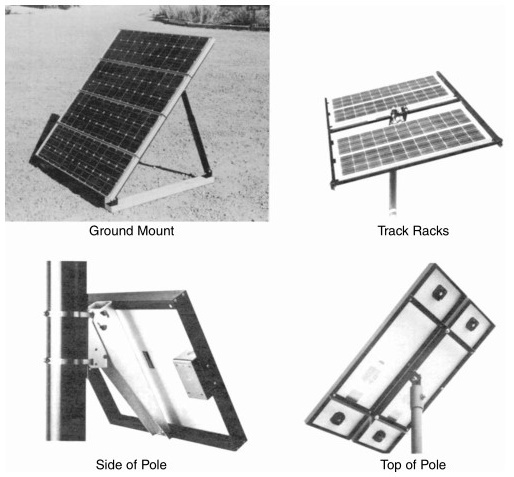
\includegraphics[scale=0.6]{./image/Mount_Method.jpg}
\caption{Tipos de Montagem \cite{book_2}}
\end{figure}
Pelo mapa abaixo, podemos determinar os locais mais aptos para aplicar esta tecnologia, Portugal como vemos não é das mais favoravies, também notamos que onde passa a linha de equador é onde podemos tirar maior proveito, ou seja maior {$\bf KW/m^2$}.
\begin{figure}[H]
	\centering
	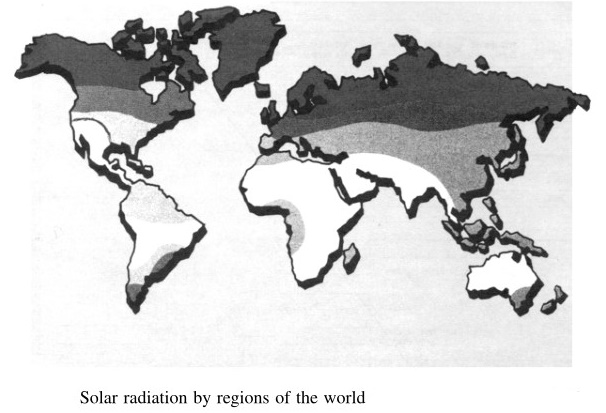
\includegraphics[scale=0.6]{./image/World_Solar_Radiation.jpg}
	\caption{Solar radiation by region of the world \cite{book_2}}
\end{figure}
\newpage

\qquad Os painéis fotovoltaicos tem vários parâmetros que determinam sua eficiência, a temperatura de funcionamento, otimização da carga, sua orientação e até limpeza são alguns pormenores, este estado de arte apenas é uma tentativa de melhor garantir tirar maior proveito da energia coletada pelo meio de orientação.\\
\\
\fbox{
\begin{minipage}{0.5\linewidth}\vspace{0pt}
\begin{figure}[H]
	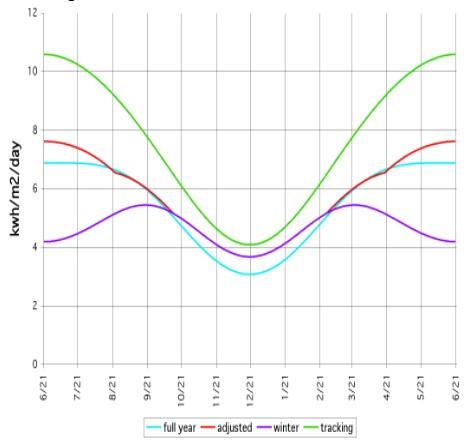
\includegraphics[scale=0.6]{./image/Graph/Anualkwh_1.jpg}
	\caption{Resposta a inclinação}
\end{figure}
\end{minipage}
}
\hspace{0.2cm}
\begin{minipage}[!t]{0.5\linewidth}
\flushleft
 Neste gráfico podemos ver um exemplo da diferença entre o rendimento de sistemas sem controlo de orientação, orientação parcial e total.\\
\vspace{7cm}
\end{minipage}\\
\\
\\
Mais energia pode ser coletada ao fim do dia se o Painel fotovoltaico tiver instalado um sistema de orientação solar, através de um atuador mecânico.\\
Existe dois tipos de sistemas de orientação solar:\cite{book_2}
\begin{enumerate}
	\setlength\itemsep{-0.1em}
	\item Sistema de um eixo, este segue o posicionamento do sol durante o dia de Este a Oeste.
	\item Sistema de dois eixos, o mesmo que de um eixo mais a orientação Norte e Sul que tem  em consideração a influencia de inclinação provocada pelas estações do ano.
\end{enumerate}




%%%%%%%%%%%%%%%%%%%%%%%%%%%%%%%%%%%%%%%%%%%%%%%%%%%%%%%%%%%%%%%%%%%%%%%%%%%%
\section{Estado da Arte}
\qquad O projeto em causa pertence a disciplina de Laboratório de Sistemas que da continuidade as disciplinas de Sistemas Digitais, sendo o foco processadores, micro-controladores e {\it Fpga´s} (Field programmable arrays). Um Micro-controlador da {\it ATmel} é o que vai ser usado como o cérebro do sistema, o tipo de sistema de orientação vai ser de um eixo, um servo motor para simulação de posicionamento e dois sensores LDR (Light dependent resitor) ligados a uma ponte wheatstone e amplificador de instrumentação para ajusto fino. Um RTC (Real Time Clock) como ferramenta de posicionamento principal, disponível um override manual, sendo seus dados visíveis num LCD (Liquid crystal display), o motor a ser usado se for numa aplicação real seria de corrente continua com íman permanente \cite{book_1} de preferência, com uma caixa redutora e sem fim para que quando estivesse em estado de paragem poder se desligar sem perder sua posição, já que se sabe que a melhor maneira de poupar energia é não a gastar. Como o objetivo é obter o maior rendimento possível pretende-se não desperdiçar, se houve-se meio de não usar energia para seu posicionamento seria o ideal.\\
No mundo das energias renováveis só é justificado sua implementação se for em grande escala pois seus rendimentos são baixos e intermitentes, e melhor ainda se os preços forem atrativos, a não ser que haja algum avanço tecnológico de relevo.\\
\\


A sun-tracking design can increase the energy yield up to 40\% over the year compared to the fixed-array design. Dual-axis tracking is done by two linear actuator motors, which follow the sun within one degree of accuracy (Figure 9.19). During the day, it tracks the sun east to west. At night it turns east to position itself for the next morning’s sun. Old trackers did this after sunset using a small nickel-cadmium battery. The new design eliminates the battery requirement by doing the turning in the weak light of the dusk and/or dawn. The Kelly cosine presented in Table 9.1 is useful in assessing accurately the power available in sunlight incident at extreme angles in the morning or evening. When a dark cloud obscures the sun, the tracker may aim at the next brightest object, which is generally the edge of a cloud. When the cloud is gone, the tracker aims at the sun once again, and so on and so forth. Such sun hunting is eliminated in newer sun trackers. \cite{book_2}\\

\newpage

\begin{figure}[H]
	\centering
	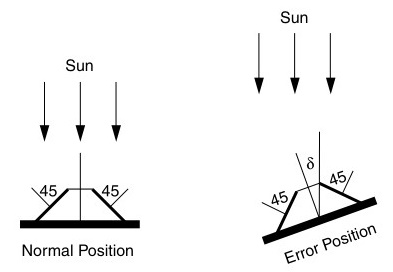
\includegraphics[scale=0.52]{./image/Sensor_Actuator_Principle.jpg}
	\caption{Principio de Funcionamento Sensor \cite{book_2}}
\end{figure}

One method of designing the sun tracker is to use two PV cells mounted on two 45° wedges , and connecting them differentially in series through an actuator motor. When the sun is normal, the currents on both cells are equal to $I_o \cos (45^o)$. \\

As they are connected in series opposition, the net current in the motor is zero, and the array stays put. On the other hand, if the array is not normal to the sun, the sun angles on the two cells are different, giving two different currents as follows: \\
$I_1 = I_o \cos(45 + \delta) and I_2 = I_o \cos(45 - \delta)$ \\
The motor current is therefore: \\
$I_m = I_1 - I_2 = I_o \cos(45 + \delta) - I_o \cos(45 - \delta)$ \\
We can express the two currents as follows: \\
$I_1 = I_o \cos (45) - I_o \delta \sin (45) and I_2 = I_o \cos (45) + I_o \delta sin (45)$ \\
The motor current is then\\
\\
$I_m = I_1 - I_2 = 2 I_o \quad \delta \sin (45) = \sqrt{2} I_o \delta \quad if \quad \delta \quad is \quad in \quad radians$ \\
A small pole-mounted panel can use one single-axis or dual-axis sun tracker. A large array, on the other hand, is divided into small modules, each mounted on its own sun tracker. This simplifies the structure and eliminates the problems related to a large movement in a large panel.



\newpage

The battery stores energy in an electrochemical form and is the most widely used device for energy storage in a variety of applications. The electrochemical energy is in a semiordered form, which is in between the electrical and thermal forms. It has a one-way conversion efficiency of 85 to 90\%.
There are two basic types of electrochemical batteries:
The primary battery, which converts chemical energy into electric energy.\\
The electrochemical reaction in a primary battery is nonreversible, and the battery is discarded after a full discharge. For this reason, it finds applica- tions where a high energy density for one-time use is required.
The secondary battery, which is also known as the rechargeable battery.
The electrochemical reaction in the secondary battery is reversible. After a discharge, it can be recharged by injecting a direct current from an external source. This type of battery converts chemical energy into electric energyin the discharge mode. In the charge mode, it converts the electric energy into chemical energy. In both modes, a small fraction of energy is converted into heat, which is dissipated to the surrounding medium. The round-trip conversion efficiency is between 70 and 80\%.

The internal construction of a typical electrochemical cell is shown in Figure 10.1. It has positive and negative electrode plates with insulating separators and a chemical electrolyte in between. The two groups of electrode plates are connected to two external terminals mounted on the casing. The cell stores electrochemical energy at a low electrical potential, typically a few volts. The cell capacity, denoted by C , is measured in ampere-hours (Ah), meaning it can deliver C A for one hour or C / n A for n hours.
The battery is made of numerous electrochemical cells connected in a series–par-allel combination to obtain the desired battery voltage and current. The higher the battery voltage, the higher the number of cells required in series. The battery rating is stated in terms of the average voltage during discharge and the ampere-hour capacity it can deliver before the voltage drops below the specified limit. The product of the voltage and ampere-hour forms the watthour (Wh) energy rating the battery
can deliver to a load from the fully charged condition. The battery charge and discharge rates are stated in units of its capacity in Ah. For example, charging a 100-Ah battery at C
/10 rate means charging at 100/10 = 10 A. Discharging that
battery at C /2 rate means drawing 100/2 = 50 A, at which rate the battery will be fully discharged in 2 h. The state of charge ( SOC ) of the battery at any time is defined as the following:
FIGURE 10.1
Electrochemical energy storage cell construction.
$SOC = \frac{Ah capacity remaning in the battery}
{Rated Ah capacity}$





\newpage




\newpage

\begin{minipage}[t]{.60\linewidth}
	%	\quad List 1:
	\begin{itemize}
		\setlength\itemsep{-0.3em}
		\item ET-BASE AVR ATmega128 \\
		Mainboard com MCU atmega 128 da ETT. \\
		\item LDR - Light Controlled Resistor \\
		Dark resistance 1M.\\
		40k at 10 lux.\\
		Max voltage 100V.\\
		Max power 80mW.\\
		\item INA128PA - Instrumentation Amplifier \\
		Banda de transmissão: 1.3MHz \\
		Montagem: THT \\
		Número de canais: 1 \\
		Carcaça: DIP8 \\
		Rapidez de subida de tensão: 4V / $\mu$ s \\
		Temperatura de trabalho: -40...85°C \\
		Entradas de tensão instável: 0.025mV \\
		Tensão de trabalho: 2.25...18V \\
		\item LCD 20x4 Blue NHD-0420DZ-NSW-BBW \\
		4x20 Characters HD44780 compatible\\
	\end{itemize}
\end{minipage}
\begin{minipage}[t]{.31\linewidth}
	%	\quad List 2:
	\begin{itemize}
		\setlength\itemsep{-0.3em}
		\item Model Craft RS-2 \- Servo Motor \\
		Control System:\\
		+Pulse Width Control 1500 $\mu$ sec \\
		Operating Voltage:\\ 
		4.8-6.0 Volts \\
		Operating Speed (4.8V):\\
		0.19sec/60° at no load \\
		Stall Torque (4.8V):\\
		42 oz/in (3.0 kg/cm) \\
		\item PCF8563 RTC Board \\
		Real-time clock/calendar function. \\ 
		Battery on board. \\
		I2C communication. \\
		\item KEYPAD4X4W \\
		16 Button Keypad switch. \\
	\end{itemize}
\end{minipage}\\
{\it https://www.ptrobotics.com/} \\
{\it https://www.futurlec.com/index.shtml} \\








%\begin{figure}[H]
%\centering
%\includegraphics[scale=0.52]{./image/OB/OB_contributions.jpg}
%\caption{Contribuições para OB \cite{book_2}}
%\end{figure}
%\cite{book_10}\\
%\begin{figure}[H]
%\begin{minipage}{0.3\linewidth}
%\flushleft
%\includegraphics[scale=0.30]{./image/OB/OB_MUltilevelmodelCulture.jpg}
%\end{minipage}
%\hspace{1cm}
%\begin{minipage}{0.4\linewidth}
%\flushleft
%\includegraphics[scale=0.44]{./image/OB/Hofstede_pt}
%\end{minipage}
%\caption{Modelo de Multi-níveis \cite{book_11} da cultura e Modelo Hofstede, Portugal}
%\end{figure}
%%%%%%%%%%%%%%%%%%%%%%%%%%%%%
%\textcolor{blue}{Visão} e seus \textcolor{blue}{Valores}.\\
%%%%%%%%%%%%%%%%%%%%%%%%%%%%%
%\textcolor{blue}{missão} 
%\begin{figure}[H]
%\flushleft
%\captionsetup{justification=raggedright,singlelinecheck=false}
%\includegraphics[scale=0.4]{./image/OB/OC_Dimensions.jpg}
%\caption{Dimensões da Cultura Organizacional \cite{book_4}}
%\end{figure}\par
\newpage


















%\begin{figure}[ht]
%\begin{center}
%\includegraphics[scale=0.5]{./image/ROQ/maquinas/ECO-P18_600x600-2-275x275.jpg}
%\includegraphics[scale=0.5]{./image/ROQ/maquinas/EVO-600x600-275x275.jpg}
%\includegraphics[scale=0.5]{./image/ROQ/maquinas/nanop10-275x275.jpg}
%\includegraphics[scale=0.5]{./image/ROQ/maquinas/NEXTP18-600x6001-275x275.jpg}
%\includegraphics[scale=0.5]{./image/ROQ/maquinas/PRO-600x600-275x275.jpg}
%\includegraphics[scale=0.5]{./image/ROQ/maquinas/You-600x600-275x275}
%\end{center}
%\caption{Produtos Principais}
%\end{figure}
%%%%%%%%%%%%%%%%%%%%%%%%%%%%%%%%%%%%%%%%%%%%%%%%%%%%%%%%%%%%%%%%%%%%%%%%%%%%
\newpage
\section{Equipamento}
%%%%%%%%%%%%%%%%%%%%%%%%%%%%%%%%%%%%%%%%%%%%%%%%%%%%%%%%%%%%%%%%%%%%%%%%%%%%
%\vspace{1cm}\\
%\begin{figure}[H]
%\centering
%\includegraphics[scale=.5]{./image/OB/Leadership.jpg}\\
%\caption{Inquérito do Estilos de Liderança \cite{article_1}}
%\end{figure}\par
%%%%%%%%%%%%%%%%%%%%%%%%%%%%%%%%%%%%%%%%%%%%%%%%%%%%%%%%%%%%%%%%%%%%%%%%%%%%%%%%%%%%%%%%%%%%%%%%%%%%%%%%%%%%%%%
\newpage
%\vspace{1cm}
%\begin{figure}[H]
%\centering
%\includegraphics[scale=.6]{./image/OB/Culture.jpg}\\
%\caption{Inquérito do tipo de Cultura Organizacional \cite{article_1}}
%\end{figure}\par
%\begin{figure}[H]
%\centering
%\includegraphics[scale=.35]{./image/OB/Ogbonna_Harris.jpg}\\
%\caption{Modelo Ogbonna \& Harris \cite{article_1}}
%\label{Modelo}
%\end{figure}\par
%%%%%%%%%%%%%%%%%%%%%%%%%%%%%%%%%%%%%%%%%%%%%%%%%%%%%%%%%%%%%%%%%
\newpage
\section{Conclusões}

%%%%%%%%%%%%%%%%%%%%%%%%%%%%%%%%%%%%%%%%%%%%%%%%%%%%%%%%%%%%%%%%%%
\newpage
%%%%%%%%%%%%%%%%%%%%%%%%%%%%%%%%%%%%%%%%%%%%%%%%%%%%%%%%%%%%%%%%%%
%Figuras Bibliografia Index
\listoffigures
\cite{*}
\bibliography{./bibliography/Bibliography}
%\printindex
\newpage
\footnote{Apontamento}
\end{document}
%%%%%%%%%%%%%%%%%%%%%%%%%%%%%%%%%%%%%%%%%%%%%%%%%%%%%%%%%%%%%%%%%%
\begin{comment}
\textcolor{orange}{O}pportunity (oportunidades)
\textcolor{purple}{I}nterno
\end{comment}